\chapter{Características y limitaciones de AWS}
\section{Características}
Las características o servicios ofrecidos por AWS son los siguientes:
\begin{figure}[h]
	\centering
	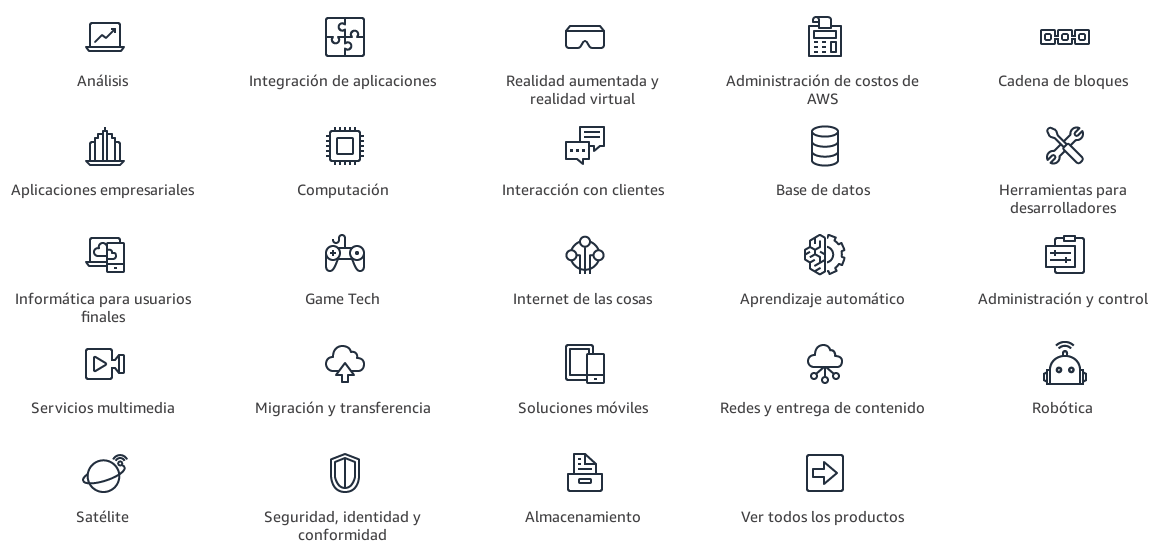
\includegraphics[scale=0.4]{ImagenesAWS/Servicios.png}
	\caption{Servicios ofrecidos por AWS.}
	\label{Servicios ofrecidos por AWS}
\end{figure}

Dentro de los servicios que podemos ver en la figura \ref{Servicios ofrecidos por AWS}, vamos a describir los más destacables:
\begin{itemize}
	\item \textbf{Amazon Elastic Cloud (EC2):} Permite la configuración y ejecución de servidores en demanda mediante un Amazon Machine Instance (AMI).
	\item \textbf{AMI:} Una imagen de Amazon machine (AMI) proporciona la información necesaria para lanzar una instancia. Debe especificar una AMI al lanzar una instancia. Cuando se necesiten varias instancias con la misma configuración, se pueden lanzar desde una misma AMI.
	
	Una AMI incluye lo siguiente:
	\begin{itemize}
		\item Una plantilla para el volumen raíz de la instancia (por ejemplo, un sistema operativo, un servidor de aplicaciones y las aplicaciones necesarias).
		\item Permisos de lanzamiento que controlan qué cuentas de AWS pueden utilizar la AMI para lanzar instancias.
		\item Un mapeo de dispositivos de bloques que especifica los volúmenes que se van a adjuntar a la instancia cuando se lance.
	\end{itemize}
	\item \textbf{Amazon Simple Storage Service (S3):} Permite guardar y recuperar datos en la nube.
	\item \textbf{Amazon Simple DB:} Proporciona funcionalidad de una base de datos sobre una máquina Amazon S3 basada en pares clave-valor.
	\item \textbf{Amazon Simple Queue Service (SQS):} Servicio de mensajería para encolar tareas y mensajes.
	\item \textbf{Amazon Relational Database Service (RDS):} Servicio web para crear, operar y escalar una base de datos en la nube.
	\item \textbf{Amzaon CloudFront:} Una copia de sus objetos más populares son cacheados en una red de nodos alrededor del mundo.
\end{itemize}

En cuanto al resto de servicios, AWS ofrece todo tipo de herramientas y aplicaciones para desarrolladores, empresas, Internet de las cosas (IoT), gestión de usuarios, robótica, redes y servicios multimedia.

\section{Limitaciones}
Dentro de la capa de estudiantes\footnote{La que hemos podido probar gracias al acuerdo de la UCA con Amazon.} tenemos las siguientes limitaciones (entre muchas más):
\begin{itemize}
	\item \textbf{Amazon EC2:} Tiene límites tanto sobre el tipo de instancia que puede utilizar como la cantidad de horas que puede utilizar en un mes.
	\item \textbf{Amazon S3:} Tiene un límite en la cantidad de almacenamiento que puede utilizar y sobre la frecuencia con al que puede llamar a determinadas operaciones cada mes.
	\item \textbf{Amazon RDS:} Tiene un límite de 750 horas al mes durante los primeros 12 meses tanto para linux como para windows en cualquier combinación de instancias. Encender una máquina una vez, hará que cuente como una hora, por lo que es más recomendable iniciarla durante 3 horas (contabilizará 3 horas), que iniciarla 3 veces en una hora (también contabilizará 3 horas).
\end{itemize}

En cuanto a servicios, podemos echar en falta aquellos relacionados con la Inteligencia Artificial, o aplicaciones que hagan uso de Inteligencia Artificial en su procesamiento.